
%\section{USER STUDY}
%There are two studies.
%The purpose of the study is to determine users� ability to provide 2D input using FingerPad. 


%Two usage conditioned were included: seated and walking.
%Our goal was to understand how precise the participants can perform cursor control on the move.


\subsection{USER STUDY}

The purpose of the study is to determine users' ability to provide precise cursor control through the fingertips in pinch. 
Because the subtle interactions are designed for mobile usage, therefore, the seated and walking conditions are considered. 
The walking condition allows us to see the level of influence while using the FingerPad technique on the move with glass displays.
Moreover, the committed methods may also affect users' performance. 
Therefore, we not only tested flick method, but also tested bi-manual clicker method. 
Finally, we also want to know how small the target that the users can point at to know the limitation.  

%We performed the task under two conditions: seated and walking conditions. 
%The seated condition allows us to see how well participants used our techniques after training. 

%The walking condition reveals the level of influence from walking waving.
%A questionnaire followed the study.

%native user ability in cursor control because the button-press minimizes  the errors from commitment methods. 
\subsection{Task and Conditions}

The participants need to move the cursor over the target shown in the screen and commit the selection by using single-handed flick selection method or the bimanual clicker method with the non-pointing hand depending on the conditions. 
The target's color will be changed when the cursor is entered into the target square. 
Upon successful selection, the target will disappear and next target will be showed up on the screen.
We measured task time and error rate for the target sizes of 10mm, 5mm, 2.5mm, 1.2mm and 0.6mm separately. 
The 0.6mm case is included to test the users' limitation.

In the \emph{seated condition}, the participants sat on the chair in front of the table where the screen was positioned toward the them. 
They were instructed to adjust the chair height such that they could rest their dominant hands on the table for support (Figure \ref{fig:walking}a). 
The participants ensured that they could see the smallest 0.6mm target clearly. Otherwise we moved the screen closer to the participants. 
In the \emph{walking condition}, they performed the tasks on the treadmill. 
The screen was placed on top of the treadmill control platform, as shown in Figure \ref{fig:walking}b.
The treadmill was set to normal walking speed (3.5 km/hour). % with a range of 0.5km according to the participants difference. 

\begin{figure}
\begin{center}
  \begin{tabular}{@{\hspace{0.1cm}}c}
		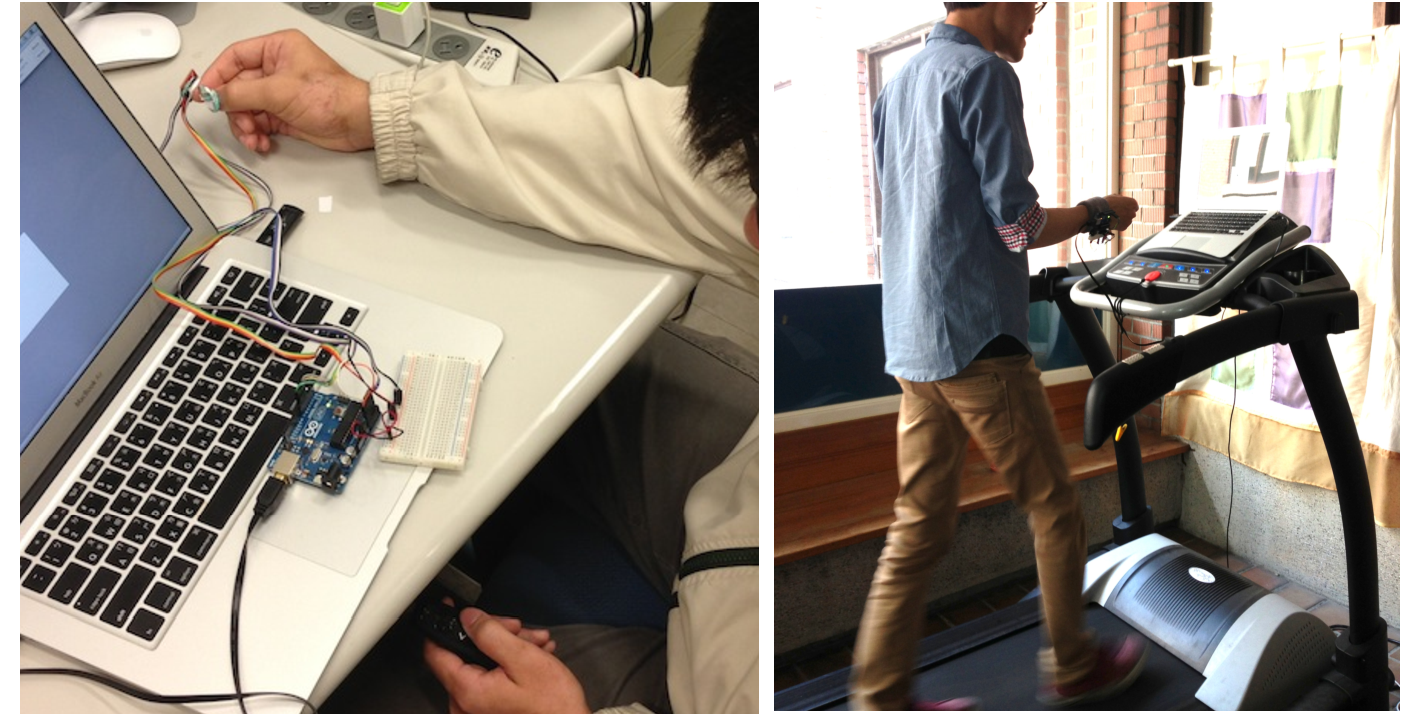
\includegraphics[width=1\linewidth]{walking3}\\
   \end{tabular}
\caption{The study setup for the seated (left) and walking conditions (right).}
\label{fig:walking}
\end{center}
\end{figure}

%\begin{figure}
%\begin{center}
%  \begin{tabular}{@{\hspace{0.1cm}}c}
%		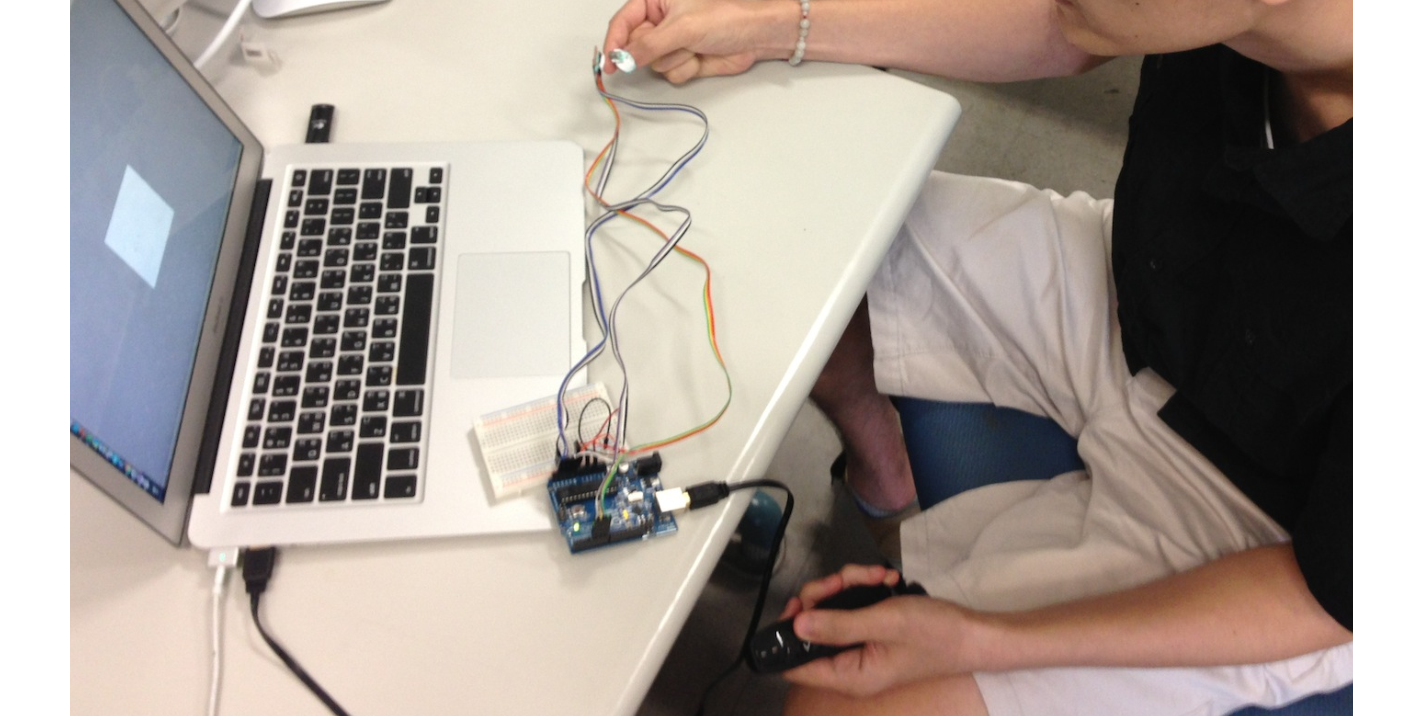
\includegraphics[width=1\linewidth]{seated3}\\
%   \end{tabular}
%\caption{The setup of our user study. (a) The screen, (b) the FingerPad device, and (c) the clicker in the non-dominant hand.}
%\label{fig:seated}
%\end{center}
%\end{figure}

\subsection{Interface and apparatus}

The participants wore the sensor part of the finger pad device on the index fingernail, and the magnet part on the thumbnail. 
Because the nail sizes and the way participants move their thumbs on the index finger pads are bio-mechanically different, we helped participants put on the device, and adjusted the magnet holder orientation in order to accommodate interpersonal tapping habits.
In the pilot testing, we found the thick fingers from some male participants could degrade the tracking performance with the original magnet setting. 
To avoid the tracking errors in the study, we replace the magnet with a wider magnet (4mm disk * 8mm height) that ensures the tracking performance in the study.
%In addition, we used a larger magnet (4mm disk * 8mm height) in the study. The stronger magnetic field makes sure participants with thicker fingertips work well, and improves cursoring stabilization.

\subsection{Experimental design}
%The experiment was a 5x2 within-subjects factorial design, with five button size conditions ( 11mm, 5.5mm, 2.8mm, 1.2mm, 0.6mm), and two commitment conditions (single-handed flick and bimanual click).
The study design was 2 x 2 x 5 x 12 (Condition x Commitment method x Target Size x Target Position) with 3 repetitions for each cell. The Condition was the between-subject variable. The target sizes were 10mm, 5mm, 2.5mm, 1.2mm and 0.6mm separately, and the  target positions were the 12 centroids of a regular 4 x 3 grid. 
For each trial, we recorded the task completion time and error. 
The different commit methods were counterbalanced. 
The target sizes and positions were randomized. %Participants received up-front training.

\subsection{Participants}
22 participants (10 female) with mean age of 26.9 (std: 3.9), between ages of 22 and 38, were recruited from the university. 
Each was rewarded a small gift for their participating. 
The task took about 30 minutes. 
All participants have the experience of touching input, because they all have touch-input smart phones.
All are right-handed.


\begin{figure}
\begin{center}
  \begin{tabular}{@{\hspace{0.1cm}}c}
		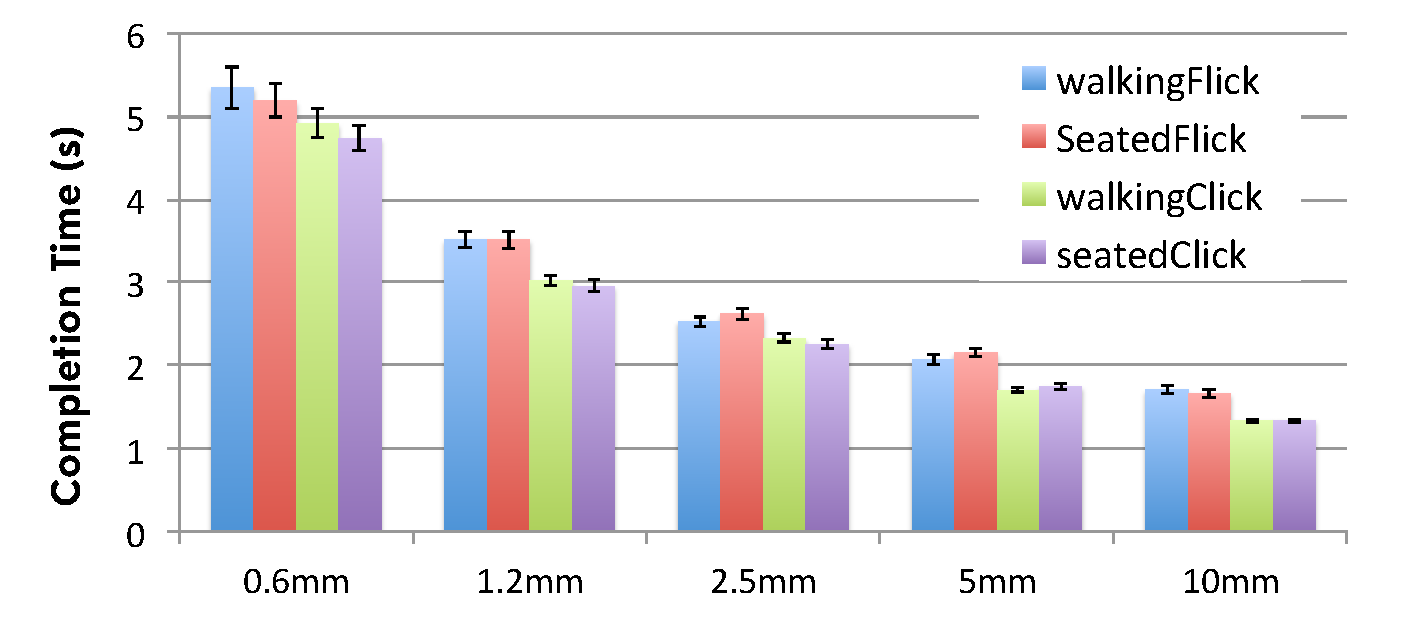
\includegraphics[width=1\linewidth]{completionTime}\\
   \end{tabular}
\caption{The study completion times, with 95\% confidence intervals, of different target sizes in two commitment methods under seated and walking conditions.}
\label{fig:completionTime}

\end{center}
\end{figure}
\begin{figure}
\begin{center}
  \begin{tabular}{@{\hspace{0.1cm}}c}
		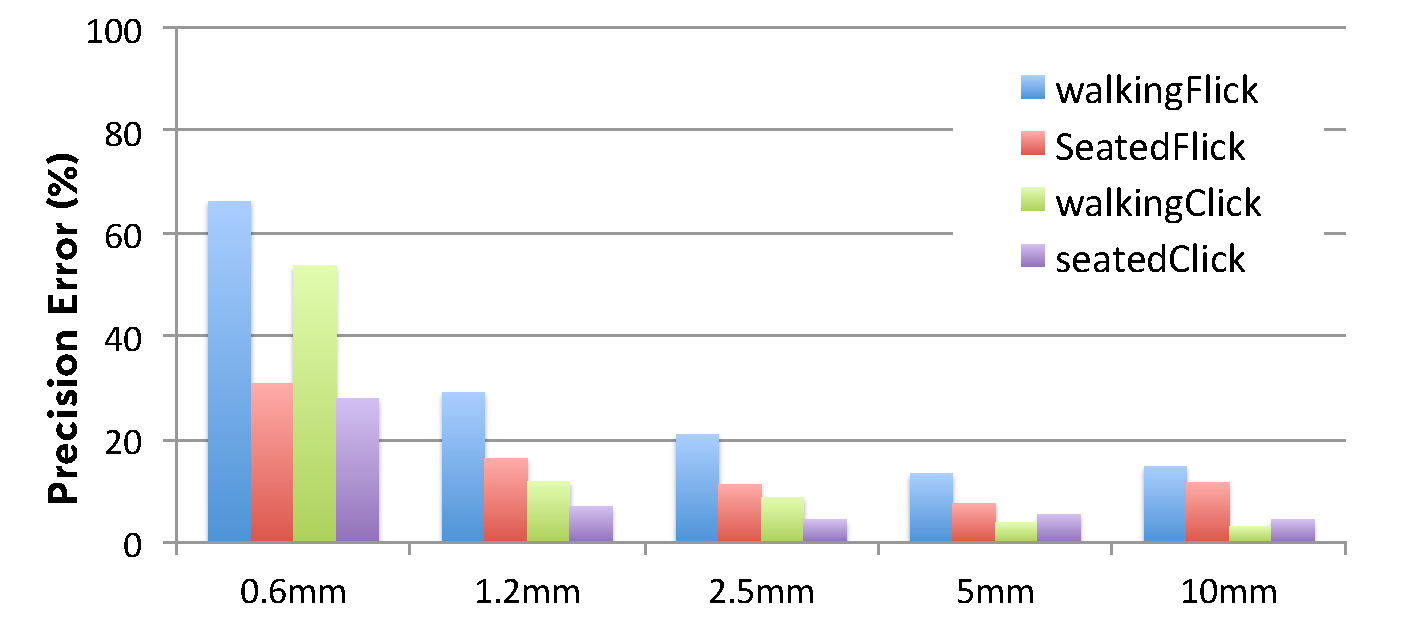
\includegraphics[width=1\linewidth]{errorRate}\\
   \end{tabular}
\caption{The study error rates of different target sizes in two commitment methods under seated and walking conditions.}
\label{fig:errorRate}
\end{center}
\end{figure}


\subsection{Results and discussion}
%For four different conditions (i.e. walkingFlick, walkingClick, seatedFlick, and seatedClick), the smaller the target size, the more time participants needed to take to complete the task (M = 1.5s for 10.0mm, 1.9s for 5.0mm, 2.4s for 2.5mm, 3.2s for 1.2mm, and 4.9s for 0.6mm across all conditions). 

%There were no significant difference between four conditions for target size 0.6mm, 1.2mm, 2.5mm. While for the target size of 5.0mm, the post host Bonferroni test showed that there were not significant between �seating� and �walking� conditions for both flick (M = 0.07s v.s. 0.13s, p = 0.30) and click (M = 0.05s v.s. 0.04s, p = 3.66) commitment approaches. 
%For the target size of 10.0mm, similar results had been discovered (M = 0.11s v.s. 0.14s, p = 0.10 for flick. M = 0.05s v.s. 0.03s, p = 3.81 for click).

%There were no significant differences (p < .05?) between the seated and walking conditions.
 

%%% Same size: Same interaction method: different posture: compare the complete time & error rate 

\subsubsection{With the same target size, the same commitment method, but different postures}

To analyze the obtained data, we ran the t-test pairwisely to know whether the different postures will affect the users' performance. 
The statistics shows that no matter the condition is walking or seated, the completion time has no significant difference. 
However, for error rate, when the target size is below 2.5mm, it shows the significant difference between the two different postures. 
For the design insight, if the system can detect users' postures, it can provide different UI layouts when users are in different postures. 
For example, while users are seated, the system can provide tight layout and compact information, and while users are walking, the system can provide loose layout and abstract information. 
However, if the users want  the consistent user experience, the target size should be above 2.5 mm.


%%% Same size: different interaction method: same posture: compare the complete time & error rate 

\subsubsection{With the same target size, the same posture, but different commitment methods}

To analyze the obtained data, we ran the t-test pairwisely to know whether the different commitment methods will affect the users' performance. 
For the completion time, the statistics shows that there is a significant difference only in the condition while the posture is walking and the target size is 10mm.
Therefore, we can say that generally the two different commitment postures don't affect the performance of the completion time. 
On the contrary, for the error rate, except the 0.6mm case, while in the walking condition, the statistics shows significant difference between flick and clicker methods. 
For the design insight, we can conclude that if we want to improve the performance, we can choose the different commitment methods. 
However, there is a trade-off between the two methods. 
Though the clicker method can achieve better performance, it requires bimanual interaction. 
Compared to clicker method, users can performance the task with only one hand, which provides more freedom to the other hand.

\subsubsection{With the same commitment method, the same posture, but different target sizes}

To analyze the obtained data, we ran the t-test pairwisely to know whether the different target sizes will affect the users' performance. 
No matter in completion time or error rate, the statistics shows that 0.6mm has significant difference compared to all the other target sizes while the posture is walking or seated. 
For the completion time, it further shows that 1.2mm has significant difference compared to 5mm and 10mm while the posture is walking or seated. 
Hence, for the design insight, 
%we can say that while the button is smaller than 0.6mm, we can call it as small button, and while the button is above 1.2mm, we can call it as large button. 
we suggest the button size should be larger than 1.2mm for better user experience.
Though the different commitment methods can achieve different performance, we doubt that it is hard to improve the performance in any commitment method while the button's size is under 0.6mm. 


%completion time:
%walking/flick: 0.6mm has sig diff to all the other
%1.2mm : 5/10
%
%waling/click: 0.6mm for all
%1.2mm: 2.5/5/10
%2.5mm: 10
%
%seated/flick: 0.6 for all
%1.2mm: 5/10
%
%seated/click: 0.6 for all
%1.2mm: 5/10
%2.5: 10
%
%error rate:
%waling/flick: 06mm for all
%1.2mm: 5/10
%
%walking/click: 06mm for all
%
%seated/flick: 06mm for all
%
%seated/click: 06mm for all


%
%As shown in Figure \ref{fig:completionTime} and Figure \ref{fig:errorRate}, the clicker method performs better in higher accuracies and shorter completion time than the flick method. In the seated condition, the flick method achieves accuracies approximately 90\% for 10mm width targets, but drops rapidly for the smaller targets. For the flick selection, participants reported they felt unconfident by taking off the thumb for selection, even if they were familiar with the selection technique. But they also reported single-handed selection is a desirable feature, in comparison to the bimanual clicker.
%
%From the results of the clicker method, participants were able to achieve accuracies in excess of 93\% in the seated condition for square targets with widths of 1.2mm , and 92\% in the walking condition for targets with widths of 2.5mm.
%The error rates increased at the widths of 0.6mm in both conditions, where the walking condition was about two times worse than seated condition. 

Though the user study, we were also impressed by the users' ability in cursor control under walking condition, even though the cursor jittering was inevitable.
When working on the smallest target, the participants reported that they reduced the jittering by pressing hard with the pinch gesture. 
For the details, they first moved the cursor to the target nearby, then added force between the fingertips, and slightly moved the cursor's position for fine control.

Generally, through the user studies, we can conclude three design insights.
First, the different postures indeed affect the performance, but while the target size is larger enough, e.g., larger than 2.5mm, the influence is diminished significantly. 
Second, the different commitment methods can achieve different performance. By considering the comfortableness and convenience, the alternative designs of the single-handed commitment methods can also be considered. For example, hard pressing Figure \ref{fig:clickMethods}a, moving the middle finger in the air Figure \ref{fig:clickMethods}b, or slightly twisting the wrist Figure \ref{fig:clickMethods}c can be the method.
Third, the target size of the control buttons should not be too small, e.g., smaller than 0.6mm. 
Nevertheless, the system design should consider the trade-off among the three factors.  






%\subsubsection{Other commitment methods}
%When asked other commitment methods for FingerPad, in sum, participants reported two kinds of other single-handed methods, as shown in Figure \ref{fig:clickMethods}. The first is simply pressing in the pinch gesture for selection, akin to the use of the computer mouse. The other is to commit by moving other parts of the operation hand, such as moving the middle finger in the air, or slightly twisting the wrist for commitment.. 

\begin{figure}
\begin{center}
  \begin{tabular}{@{\hspace{0.1cm}}c}
		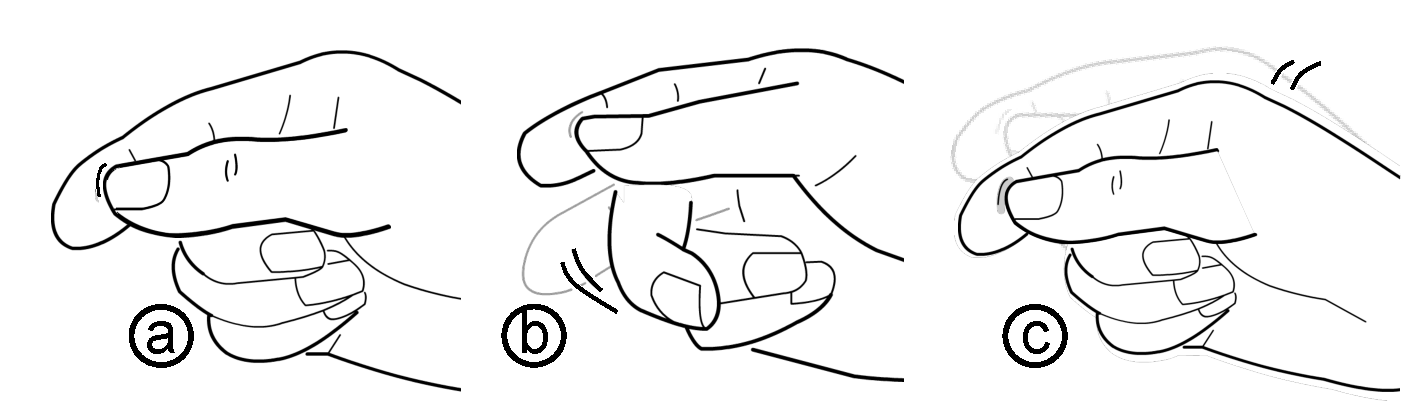
\includegraphics[width=1\linewidth]{clickMethods}\\
   \end{tabular}
\caption{Other commitment methods described by the participants. (a) press (e.g., the mouse button), (b) move the middle finger, and (c) move the wrist.}
\label{fig:clickMethods}
\end{center}
\end{figure}



